\documentclass{math}

\usepackage{graphicx}
\usepackage{listings}
\lstset{basicstyle=\ttfamily\footnotesize,breaklines=true}

\title{Introduction to Cryptography}
\author{Alvin Lin}
\date{January 2018 - May 2018}

\begin{document}

\maketitle

\section*{Public Key Cryptosystems}

\subsection*{Properties of Symmetric Key Cryptography}
\begin{itemize}
  \item The same secret key is used for encryption and decryption.
  \item Encryption and decryption are very similar (or even identical
  functions).
  \item Symmetric algorithms like AES or 3DES are secure, fast, and widespread
  but face a key distribution problem. The secret key must be transported
  securely because the security depends on the key.
  \item In a network of users, each pair of users requires an individual key.
  \( n \) users in a network would require \( \frac{n(n-1)}{2} \), where each
  user stores \( n-1 \) keys.
  \item Two users can cheat each other since they have identical keys.
  Non-repudiation is not guaranteed by symmetric key cryptography.
\end{itemize}

\subsection*{Asymmetric Key Cryptography}
The idea behind asymmetric key is similar to the idea of a mailbox. Anyone can
drop a letter into it, but only the owner can open it. The first publication of
such an algorithm was made by Whitfield Diffie and Martin Hellman in 1976. In
principle, the key is split up into a public key \( K_{pub} \) and a private key
\( K_{pr} \). This allows for mechanisms such as:
\begin{itemize}
  \item \textbf{Key Distribution}, like the Diffie-Hellman key exchange,
  without the need for a pre-shared secret.
  \item \textbf{Nonrepudiation and Digital Signatures} to prove message
  integrity.
  \item \textbf{Identification} using challenge-response protocols with
  digital signatures.
  \item \textbf{Encryption} using algorithms like RSA, though it is
  computationally expensive and 1000 times slower than symmetric algorithms.
\end{itemize}
In practice, hybrid systems are used, incorporating both asymmetric and
symmetric algorithms. Key exchanges and digital signatures are performed using
asymmetric algorithms, while data encryption is done using fast symmetric
ciphers.

\subsection*{Public Key Algorithm Theory}
Asymmetric schemes are based on some one-way function \( f \), where computing
\( y = f(x) \) is computationally easy, but computing \( x = f^{-1}(y) \) is
computationally infeasible. One way functions are usually based on
mathematically difficult problems, such as:
\begin{itemize}
  \item \textbf{Factoring Integers}: given a composite integer \( n \), find its
  prime factors.
  \item \textbf{Discrete Logarithm (DL)}: given \( a,y,m \), find \( x \) such
  that \( a^x = y\mod m \).
  \item \textbf{Elliptic Curves (EC)}: generalization of discrete logarithm.
\end{itemize}

\subsubsection*{Key Lengths and Security Levels}
\begin{center}
  \begin{tabular}{|c|c|c|c|}
    \hline
    Symmetric & ECC & RSA, DL & Remark \\
    \hline
    64 bit & 128 bit & \( \approx \) 700 bit & short term security \\
    \hline
    80 bit & 160 bit & \( \approx \) 1024 bit & medium security \\
    \hline
    128 bit & 256 bit & \( \approx \) 3072 bit &  long term security \\
    \hline
  \end{tabular}
\end{center}
The exact complexity of RSA and DL is difficult to estimate. The existence of
quantum computers would probably be the end for ECC, RSA, and DL, but that is
still decades away. Some researchers doubt that quantum computers will ever
exist.

\subsubsection*{Euclidean Algorithm}
Earlier, we explored the Euclidean algorithm for finding the greatest common
divisor, which is based on the observation that:
\[ gcd(r_0) = gcd(r_0-r_1,r_1) \]
By reducing the problem recursive, we find that \( gcd(r_i,0) = r_i \) is the
answer to the original problem. We can extend the Euclidean algorithm to find
the modular inverse of \( r_1 \mod r_0 \). In order for the inverse to exist:
\[ gcd(r_0,r_1) = 1 \]
The extended Euclidean algorithm computes \( s,t \) such that:
\[ gcd(r_0,r_1) = s\cdot r_0+t\cdot r_1 = 1 \]
If we take this relation mod \( r_0 \):
\begin{align*}
  s\cdot r_0+t\cdot r_1 &= 1
  s\cdot r_0+t\cdot r_1 \equiv 1\mod r_0 \\
  t\cdot r_1 &\equiv 1\mod r_0
\end{align*}
By definition, \( t \) is the inverse of \( r_1 \mod r_0 \).

\subsubsection*{Euler's Phi Function}
Euler's Phi function \( \phi(m) \) gives the numbers in the set of integers from
0 to \( m-1 \) that are relatively prime to \( m \). Example:
\begin{align*}
  gcd(0,6) = 6 \\
  gcd(1,6) = 1 \\
  gcd(2,6) = 2 \\
  gcd(3,6) = 3 \\
  gcd(4,6) = 2 \\
  gcd(5,6) = 1 \\
  \phi(6) = 2
\end{align*}
\( \phi(6) = 2 \) since only 1 and 5 are relatively prime to \( m = 6 \). If the
canonical factorization (prime factorization) of \( m \) is known, where:
\[ m = p_1^{e_1}\cdot p_2^{e_2}\cdot\dots\cdot p_n^{e_n} \]
such that \( p_i \) are primes and \( e_i \) are positive integer exponents,
then \( \phi(m) \) can be calculated by:
\[ \phi(m) = \prod_{i=1}^{n}(p_i^{e_i}-p_i^{e_i-1}) \]
For example:
\begin{align*}
  m &= 12 = 2^2\cdot3^1 \\
  \phi(12) &= (2^2-2^1)\cdot(3^1-3^0) = 4 \\
  m &= 899 = 29^1\cdot31^1 \\
  \phi(899) &= (29^1-29^0)\cdot(31^1-31^0) = 38\cdot30 = 840
\end{align*}
Finding \( \phi(m) \) is computationally easy if the factorization of \( m \) is
known, otherwise it becomes computationally infeasible for large numbers.

\subsubsection*{Fermat's Little Theorem}
Given a prime \( p \) and an integer \( a \) such that \( a^p \equiv a\mod p \),
the following is true:
\[ a^{p-1} \equiv 1\mod p \]
This is used to find the modular inverse if \( p \) is prime. We can rewrite
the relation above as follows:
\begin{align*}
  a^{p-1} &\equiv 1\mod p \\
  a\cdot a^{p-2} &\equiv 1\mod p
\end{align*}
By the definition of the modular inverse:
\begin{align*}
  a\cdot a^{-1} &\equiv 1\mod p \\
  a^{-1} &\equiv a^{p-2}\mod p
\end{align*}
For example, \( a = 2, p = 7 \):
\begin{align*}
  2^7 &\equiv 2\mod7 \\
  2^{-1} &\equiv 2^5\mod7 \equiv 4\mod7 \\
  2\cdot4 &\equiv 1\mod 7
\end{align*}

\subsection*{The RSA Cryptosystem}
After Martin Hellman and Whitfield Diffie published their public key paper in
1976, Ronald Rivest, Adi Shamir, and Leonard Adleman proposed the asymmetric
RSA cryptosystem in 1977. Until now, RSA was the most widely used asymmetric
cryptosystem, with elliptic curve cryptography gaining popularity. It has two
main applications, the transport of symmetric keys, and digital signatures.
RSA operations are done over the integer ring \( Z_n \) where \( n = pq \)
such that \( p \) and \( q \) are large primes. Encryption and decryption are
simply exponentiations in the ring. Given the public key \( (n,e) = k_{pub} \)
and the private key \( d = k_{pr} \):
\begin{align*}
  y &= e_{k_{pub}}(x) \equiv x^e\mod n \\
  x &= d_{k_{pr}}(y) \equiv y^d\mod n
\end{align*}
where \( x,y \in Z_n \). In practice, \( x,y,n,d \) are very long integer
numbers, usually greater than 1024 bits. The security of the scheme relies on
the fact that it is hard to derive the private exponent \( d \) given the
public key \( (n,e) \).

\subsubsection*{Key Generation}
Like all asymmetric schemes, RSA has set up phases during which the private and
public keys are computed. To generate an rsa key pair:
\begin{enumerate}
  \item Choose two large primes \( p,q \)
  \item Compute \( n = pq \)
  \item Compute \( \phi(n) = (p-1)(q-1) \)
  \item Select the public exponent \( e\in\{1,2,3,\dots,\phi(n)-1\} \) such that
  \( gcd(e,\phi(n)) = 1 \).
  \item Compute the private key \( d \) such that \( de \equiv 1\mod\phi(n) \)
  \item \( k_{pub} = (n,e) \quad k_{pr} = d \)
\end{enumerate}
Choose the two large distinct primes \( p,q \) in step 1 is non trivial. Step
4, ensures that \( e \) has an inverse and thus there is always a private key
\( d \).

\subsubsection*{Implementation Aspects}
The RSA cryptosystem uses only one arithmetic operation (modular
exponentiation), which makes it conceptually a simple asymmetric scheme. Even
though it is conceptually simple, it is orders of magnitude slower than
symmetric schemes such as DES or AES due to the use of very long numbers.
When implementation RSA on devices with memory constraints, arithmetic
algorithms must be selected very carefully.

\subsubsection*{The Square and Multiply Algorithm}
The square and multiply algorithm allows for fast exponentiation for very long
numbers. This is done by converting the exponent to binary and squaring or
multiplying the base depending on the current bit of the exponent. Modular
reduction can be applied during each step to keep the operands small. Example
for \( x^{26} \) (without modular reduction):
\[ 26 = (11010)_2 \]
\begin{center}
  \begin{tabular}{|c|c|c|c|}
    \hline
    Step & Accumulated Result & Binary Exponent & Operation \\
    \hline
    1 & \( r = (1^2)x = x \) & 1 & Square and Multiply \\
    \hline
    2 & \( r = (x^2)x = x^3 \) & 11 & Square and Multiply \\
    \hline
    3 & \( r = (x^3)^2 = x^6 \) & 110 & Square \\
    \hline
    4 & \( r = (x^6)^2x = x^{13} \) & 1101 & Square and Multiply \\
    \hline
    5 & \( r = (x^{13})^2 = x^{26} \) & 11010 & Square \\
    \hline
  \end{tabular}
\end{center}
This algorithm has a logarithmic complexity since its run time is proportional
to the bit length of the exponent. Given an exponent with \( t+1 \) bits, we
need to perform \( t \) squarings and an average of \( 0.5t \) multiplications.
Since exponents are chosen randomly, \( 1.5t \) is a good estimate for the
average number of operations. Modular exponentiation is still computationally
expensive. For devices with memory constraints, RSA can still be quite slow.
Choosing a small public exponent \( e \) to perform RSA with does not weaken
the security of the algorihtm, but significantly improves the speed.

\subsection*{The Chinese Remainder Theorem (CRT)}
Sun Tzu, the author of \textit{The Art of War}, is said to have created the
Chinese remainder theorem as a method of counting the size of the ancient
Chinese armies. Let \( n_1,\dots,n_i,\dots,n_r \) be integers greater than 1.
If the \( n_i \) are pairwise coprime, and if \( a_1,\dots,a_r \) are integers
such that \( 0\le a_i\le n_i \) for every \( i \), then the Chinese Remainder
Theorem states that the system
\begin{align*}
  x &\equiv a_1\mod n_1 \\
  x &\equiv a_2\mod n_2 \\
  &\dots \\
  x &\equiv a_r\mod n_r
\end{align*}
has a unique solution \( x \) such that \( 0\le x<N \). Additionally, let
\( N = n_1\cdot n_2\cdot n_3\cdot\dots\cdot n_r \). Then
\[ x \equiv (a_1b_1N_1+a_2b_2N_2+\dots+a_rb_rN_r)\mod N \]
where \( N_i = \frac{N}{n_i} \) and \( b_i \) is determined from
\[ b_iN_i \equiv 1\mod n_i \]
for \( i \) from 1 to \( r \).

\subsubsection*{Example}
\begin{align*}
  x &\equiv 2\mod3 \\
  x &\equiv 3\mod5 \\
  x &\equiv 2\mod7 \\
  N &= n_1n_2n_3 = 105 \\
  N_1 &= 35 \quad N_2 = 21 \quad N_3 = 15 \\
  35b_1 &\equiv 1\mod3 \quad 2b_1 \equiv 1\mod3 \\
  21b_2 &\equiv 1\mod5 \quad 1b_2 \equiv 1\mod5 \\
  15b_3 &\equiv 1\mod7 \quad 1b_3 \equiv 1\mod7 \\
  b_1 &= 2 \quad b_2 = 1 \quad b_3 = 1 \\
  x &\equiv (2\cdot2\cdot35+3\cdot1\cdot21+2\cdot1\cdot15)\mod105 \\
  &\equiv 233\mod105 \\
  &\equiv 23
\end{align*}

\subsubsection*{Example}
\begin{align*}
  x &\equiv 0\mod3 \\
  x &\equiv 3\mod4 \\
  x &\equiv 4\mod5 \\
  N &= 3\cdot4\cdot5 = 60 \\
  N_1 &= 20 \quad N_2 = 15 \quad N_3 = 12 \\
  20b_1 &\equiv 1\mod3 \quad 2b_1 \equiv 1\mod3 \\
  15b_2 &\equiv 1\mod4 \quad 3b_2 \equiv 1\mod4 \\
  12b_3 &\equiv 1\mod5 \quad 2b_3 \equiv 1\mod5 \\
  b_1 &= 2 \quad b_2 = 3 \quad b_3 = 3 \\
  x &\equiv (0\cdot2\cdot20+3\cdot3\cdot15+4\cdot3\cdot12)\mod70 \\
  &\equiv 39
\end{align*}

\subsubsection*{Application to RSA}
With regard to its application to public key cryptography, choosing a small
private key \( d \) for RSA results in security weaknesses. \( d \) must have
at least \( 0.3t \) bits, where \( t \) is the bit length of the modulus
\( n \). However, the Chinese Remainder Theorem can be used to somewhat
accelerate exponentiation with the private key \( d \). We can replace the
computation of
\[ x^{d\mod\phi(n)}\mod n \]
by two computations:
\[ x^{d\mod(p-1)}\mod p \]
\[ x^{d\mod(q-1)}\mod q \]
where \( q \) and \( p \) are ``small'' compared to \( n \). This involves
three distinct steps.
\begin{enumerate}
  \item Transformation of the operand into the CRT domain
  \item Modular exponentiation in the CRT domain
  \item Inverse transformation into the problem domain
\end{enumerate}
For example, consider the problem \( 90^{547}\mod899 \). First we need to
transform it into the CRT domain. Transformation into the CRT domain requires
knowledge of \( p \) and \( q \). These are only known to the owner of the
private key, hence it cannot be applied to speed up encryption. The
transformation computes \( (x_p,x_q) \) which is the representation of \( x \)
in the CRT domain.
\begin{align*}
  d &= 547 \\
  n &= 899 = 29\cdot31 \\
  x_p &= x\mod p = 90\mod29 = 3 \\
  x_q &= x\mod q = 90\mod31 = 28 \\
\end{align*}
The next step is exponentiation. Given \( d_p \) and \( d_q \) such that
\( d_p\equiv d\mod(p-1) \) and \( d_q\equiv d\mod(q-1) \), one exponentiation
in the problem domain requires two exponentiations in the CRT domain.
\begin{align*}
  d_p &= 547\mod28 = 15 \\
  d_q &= 547\mod30 = 7 \\
  y_p &\equiv x_p^{d_p}\mod p = 3^{15}\mod29 = 26 \\
  y_q &\equiv x_q^{d_q}\mod q = 28^7\mod31 = 14 \\
\end{align*}
In practice, \( p \) and \( q \) are chosen to have half the bit length of
\( n \). Inverse transformation requires modular inversion twice, which is
computationally expensive.
\begin{align*}
  c_p &= q^{-1}\mod p = 31^{-1}\mod29 = 15 \\
  c_q &= p^{-1}\mod q = 29^{-1}\mod31 = 15
\end{align*}
This is assembled with \( y_p,y_q \) into the final result \( y\mod n \) in
the problem domain.
\begin{align*}
  y &\equiv \bigg[(q\cdot c_p)\cdot y_p+(p\cdot c_q)\cdot y_q\bigg]\mod n \\
  y &\equiv \bigg[(31\cdot13)\cdot26+(29\cdot15)\cdot14\bigg]\mod899 = 200
\end{align*}
The primes \( p \) and \( q \) typically change infrequently. Therefore, the
cost of inversion can be neglected because \( q\cdot c_p \) and \( p\cdot c_q \)
can be precomputed and stored. We ignore the transformation and inverse
transformation steps since their costs can be neglected under reasonable
assumptions. If we assume that \( n \) has \( t+1 \) bits, both \( p \) and
\( q \) are about \( \frac{t}{2} \) bits long. The complexity is determined by
the two exponentiations in the CRT domain. The operands are only
\( \frac{t}{2} \) bits long. For the exponentiations, we use the
square-and-multiply algorithm. This gives a total complexity of \( 1.5t \) as
well, but since the operands have half the bit length of the problem exponent,
each operation is 4 times faster.

\subsection*{Finding Large Primes}
Generating keys for RSA requires finding two large primes \( p \) and \( q \)
such that \( n = pq \) is sufficiently large. The size of \( p \) and \( q \)
is typically half the size of the desired size of \( n \). To find primes,
random integers are generated and tested for primality. The random number
generator should be non-predictable otherwise an attacker could guess the
factorization of \( n \).
\par Factoring \( p \) and \( q \) to test for primality is typically not
feasible. However, we are not interested in the factorization, we only want to
know whether \( p \) and \( q \) are composite. Primality test are typically
probabilistic. They are not 100\% accurate but their output is correct with
very high probability. A probabilistic test has two outputs:
\begin{itemize}
  \item The input is composite. This is always true if it is returned.
  \item The input is a prime. This is only true with a certain probability.
\end{itemize}

\subsubsection*{Fermat Primality Test}
The basic idea is that Fermat's Little Theorem holds for all primes. If a
number \( p' \) is found for which \( a^{p'-1}\not\equiv1\mod p' \), it is not a
prime. For certain numbers like the Carmichael numbers, this test returns a
false positive when the numbers are composite. The Fermat-Primality test is
usually implemented using a candidate number \( p' \) and a security parameter
\( s \).
\begin{lstlisting}[mathescape=true]
for i = 1 to s:
  choose a random $a\in\{2,3,\dots,p'-2\}$
  if $a^{p'-1}\not\equiv1\mod p'$ then:
    return $p'$ is composite
  return $p'$ is likely a prime
\end{lstlisting}
We call \( a \) a \textbf{Fermat witness} if it shows that \( p' \) is composite
or a \textbf{Fermat liar} if it makes the algorithm give a false result.

\subsubsection*{Miller-Rabin Primality Test}
Given the decomposition of an odd prime candidate \( p' \) as
\[ p'-1 = 2^u\cdot r \]
where \( r \) is odd, if we can find an integer \( a \) such that
\[ a^r\not\equiv1\mod p' \]
\[ a^{r\cdot2j}\not\equiv p'-1\mod p' \]
for all \( j\in\{0,1,\dots,u-1\} \), then \( p' \) is composite. Otherwise, it
is probably a prime. The Miller-Rabin primality test is also implemented
using a candidate number \( p' \) and a security parameter \( s \) such that
\( p'-1 = 2^u\cdot r \).
\begin{lstlisting}[mathescape=true]
for i = 1 to s:
  choose a random $a\in\{2,3,\dots,p'-2\}$
  $z\equiv a^r\mod p'$
  if $z\ne1$ and $z\ne p'-1$ then:
    for $j=1$ to $u-1$:
      $z\equiv z^2\mod p'$
      if $z=1$ then:
        return $p'$ is composite
    if $z=p'-1$ then:
      return $p'$ is composite
return $p'$ is likely a prime
\end{lstlisting}

\subsection*{Using RSA Securely}
\begin{enumerate}
  \item Do not use primes too close together. If the difference between \( p \)
  and \( q \) is small, then \( p \) and \( q \) are both close to
  \( \sqrt{n} \), and dividing \( n \) by odd numbers around \( \sqrt{n} \) will
  find them. \( p \) and \( q \) should be chosen at random.
  \item Be careful using a small public exponent. We would like \( e \) to be
  small so the encryption operation is efficient, but if \( e \) is small and
  the message \( m \) is small, then \( me \) may be less than \( n \) and
  the private key can be computed.
  \item Don't send the same message \( m \) encrypted with different public
  keys, each with \( e = 3 \). Using the Chinese Remainder Theorem, the
  message can be commputed.
  \item Make sure no legitimate message is ever the product of two or more
  other legitimate messages since RSA is homomorphic. The signature of the
  product message can be computed without knowing the private key.
  \item Shared factor attacks: suppose Alice choose \( p \) and \( q_A \) as
  her RSA primes and Bob chooses \( p \) and \( q_B \). If they both publish
  their RSA modules \( n_A \) and \( n_B \), \( p \) can be quickly computed
  as \( gcd(n_A, n_B) \), which allows for for an attacker to reconstruct
  both Bob and Alice's private keys.
\end{enumerate}
These attacks can all be thwarted if the message \( m \) is about the same
size as \( n \), the public operation is never performed with different public
keys on the same \( m \), and the random primes are generated with proper
randomness.

\subsubsection*{Mathematical Attacks on RSA}
Mathematical attacks on RSA typically fall into three categories:
\begin{enumerate}
  \item Factoring \( n \) into its two prime factors. This enables the
  calculation of \( \phi(n) \), which in turn allows for the private key to be
  computed.
  \item Determining \( \phi(n) \) directly without first determining \( p \) and
  \( q \). This allows for the private key to be reconstructed.
  \item Determining \( d \) directly without first determining \( \phi(n) \).
\end{enumerate}

\subsubsection*{Factoring Problem}
The general number field sieve (GNFS) is the most efficient classical algorithm
known for factoring integers larger than \( 10^{100} \). The special number
field sieve (SNFS) is a special purpose integer factorization algorithm. GNFS
was derived from SNFS. The special number field sieve is efficient for integers
of the form \( r^e\pm s \), where \( r \) and \( s \) are small.

\subsubsection*{Other Attacks on RSA}
\begin{enumerate}
  \item Hardware Fault-Based Attack: this involves inducing hardware faults in
  the processor that is generating digital signatures.
  \item Chosen Ciphertext Attacks: this type of attack exploits properties of
  the RSA algorithm.
  \item Brute Force: this involves trying all possible private keys.
  \item Timing Attacks: this involves the leaking information from the running
  time of the decryption algorithm.
\end{enumerate}

\subsection*{Diffie-Hellman Key Exchange}
The Diffie-Hellman key exchange was proposed in 1976 by Whitfield Diffie and
Martin Hellman. It is widely used in SSH, TLS, and IPSec. It is a key
exchange protocol based on the discrete logarithm problem. To use this:
\begin{enumerate}
  \item Choose a large prime \( q \).
  \item Choose an integer \( \alpha\in\{2,3,\dots,p-2\} \) such that
  \( \alpha \) is a primitive root of \( q \).
  \item Publish \( q \) and \( \alpha \).
\end{enumerate}
A number \( a \) is a primitive root modulo \( q \) if for every integer \( a \)
coprime to \( q \), there is an integer \( k \) such that \( \alpha^k\equiv
a\mod p \). \( \alpha \) is known as a generator of the multiplicative group of
integers modulo \( q \) (\( \Z_{p}^{*} \)). To do a key exchange:
\begin{enumerate}
  \item \( q \) and \( \alpha \) are shared between two parties Alice and Bob.
  \item Alice and Bob each generate a private key \( X_A < q \) and
  \( X_B < q \).
  \item Alice calculates a public key \( Y_A = \alpha^{X_A}\mod q \) while Bob
  calculates a public key \( Y_B = \alpha^{X_B}\mod q \).
  \item Alice and Bob exchange public keys in plaintext.
  \item Alice calculates a shared secret key \( K = (Y_B)^{X_A}\mod q \) while
  Bob calculates the same shared secret key using \( K = (Y_A)^{X_B}\mod q \).
\end{enumerate}
Alice and Bob end up with the same key \( K = (\alpha^{X_B})^{X_A}\mod q \equiv
(\alpha^{X_A})^{X_B}\mod q \).

\subsubsection*{Man-in-the-middle Attacks}
A malicious party (Darth) sitting between Alice and Bob can intercept the
messages and send their own public key during the key exchange to gain access
to the messages being between Alice and Bob. Alice and Bob will never directly
communicate with each other, instead proxying their messages through the
malicious middleman. This can be solved by using digital signatures to
authenticate the key exchange messages.
\begin{center}
  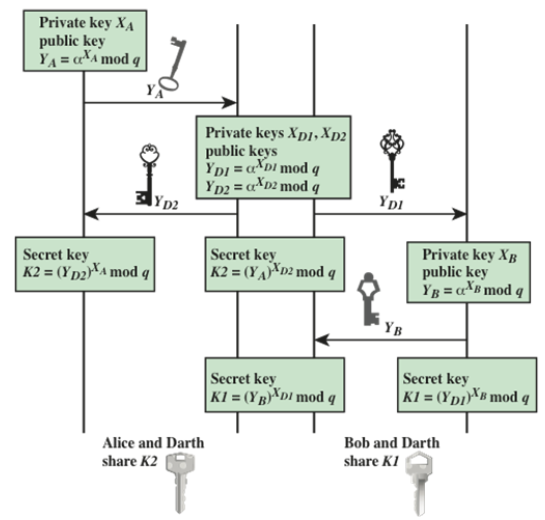
\includegraphics[width=10cm]{assets/diffie_hellman_mitm.png}
\end{center}

\subsubsection*{Multiplicative Group Modulo \( p \)}
The multiplicative group modulo \( p \) is denoted \( \Z_p^{*} =
\{1,2,\dots,p-1 \} \). The group operation is multiplication modulo \( p \) and
the group is closed under multiplication modulo \( p \). The product
\( \mod p \) of any two elements in the set is also in the set. Multiplication
is associative for any elements \( a,b,c \):
\[ a\cdot(b\cdot c) \equiv (a\cdot b)\cdot c\mod p \]
and also commutative for any elements \( a \) and \( b \):
\[ a\cdot b \equiv b\cdot a\mod p \]
1 is the identity element, and for every element \( a \) there is an inverse
\( a^{-1} \) such that \( a\cdot a^{-1}\equiv 1\mod p \). Recall from earlier
that a number \( a \) is a primitive root modulo \( q \) if for every integer
\( a \) coprime to \( q \), there is an integer \( k \) such that
\( \alpha^k\equiv a\mod p \) where \( \alpha \) is a generator of the
multiplicative group of integers modulo \( q \) (\( \Z_{p}^{*} \)).
\par An order-\( q \) subgroup of the group \( \Z_p^{*} \) is a \( q \)-element
subset of \( \{1,2,\dots,p-1\} \) such that the subset is itself a group with
the group operation being multiplication modulo \( p \). A generator of an
order-\( q \) subgroup of the group \( \Z_p^{*} \) is a number \( g \) such that
the set
\[ \{g^0\mod p, g^1\mod p,g^2\mod p,\dots,g^{q-1}\mod p\} \]
is an order-\( q \) subgroup of \( \Z_p^{*} \). If the size of the set generated
by \( g \) is \( q \), we say that the order of \( g \) is \( q \). The orders
of the subgroups of \( \Z_p^{*} \) are equal to the factors of \( p-1 \). There
is always an order-\( p-1 \) subgroup, the full group itself, and there is
always an order-1 subgroup \( \{1\} \). If \( p \) is prime, then there is
always an order-2 subgroup with generator \( p-1 \). If \( p \) is prime, then
there is always an order-\( \frac{p-1}{2} \) subgroup.

\subsection*{El Gamal Encryption}
El Gamal encryption was proposed by Taher Elgamal in 1985 as a public key
cryptosystem and a signature scheme based on discrete logarithms. It can
be viewed as an extension of the DHKE protocol based on the intractability of
the discrete logarithm problem and the Diffie Hellman problem. It begins
with the same public parameters as Diffie Hellman, a large prime \( p \),
a subgroup order \( q \), and a generator \( \alpha \) of the group
\( \Z_p^{*} \). A recipient Bob generates a key by doing the following:
\begin{enumerate}
  \item Bob picks a random number \( b \) in the range \( 1<b\le p-2 \).
  \item Bob's private key is \( X_B = b \).
  \item Bob's public key is \( Y_B = \alpha^b\mod p \).
\end{enumerate}
Alice encrypts a message \( m\in\Z_p^{*} \) for Bob by doing the following:
\begin{enumerate}
  \item The message \( m \) is padded.
  \item Alice picks a random number \( a \) in the range \( 1<a<p-2 \).
  \item Alice computes an ephemeral key \( Y_A = \alpha^a\mod p \).
  \item Alice computes a masking key \( k_M = (Y_B)^a\mod p \) from Bob's
  public key.
  \item Alice computes the ciphertext \( c = m\cdot k_M\mod p \) and sends
  \( Y_A, c \) to Bob.
\end{enumerate}
Bob decrypts the ciphertext by doing the following:
\begin{enumerate}
  \item Bob computes the masking key \( k_M = (Y_A)^b\mod p \).
  \item Bob computes the modular inverse of \( k_M\mod p \).
  \item Bob computes the original message \( m = c\cdot (k_M)^{-1}\mod p \).
\end{enumerate}

\subsection*{The Discrete Logarithm Problem}
Given the finite cyclic group \( \Z_q^* \) of order \( q-1 \) and a primitive
element \( \alpha\in\Z_q^* \) and another element \( \beta\in\Z_q^* \), the
discrete logarithm problem is the problem of determining the integer
\( 1\le x\le q-1 \) such that:
\[ a^x\equiv\beta\mod q \]

\begin{center}
  You can find all my notes at \url{http://omgimanerd.tech/notes}. If you have
  any questions, comments, or concerns, please contact me at
  alvin@omgimanerd.tech
\end{center}

\end{document}
